% ======================================================================
\section{Bodies at rest: the Cosmic Interaction Law}\label{sec:rest}
% ======================================================================

\emph{What happens when two cosmic masses meet?} This section proposes a law for a pair of bodies at rest, reads it in its own plane, and recovers Newton's and Coulomb's laws, with the sign that makes like charges push apart.

\subsection{Two numbers, two laws}\label{subsec:two-numbers}

Classical physics describes two bodies $a$ and $b$, at the distance $r$, by two numbers each: the masses $m_a$, $m_b$ in kilograms and the charges $q_a$, $q_b$ in coulombs. Along the unit arrow $\er$ from $a$ to $b$ it writes two laws of one shape, Newton's with the constant $G$ and Coulomb's with the constant $K$~\cref{eq:two-laws}. We write each force along the line as a signed number: a positive value is a pull, a negative value a push. Gravity is then $+G\,m_a m_b/r^2$, and electricity is $-K\,q_a q_b/r^2$, a push for like charges.

\subsection{The interaction law}\label{subsec:one-law}

\begin{postulate}[The Cosmic Interaction Law]\label{law:interaction}
Two bodies with the cosmic masses $\mu_a = m_a + q_a\Gp$ and $\mu_b = m_b + q_b\Gp$, at the distance $r$, interact by
\[
\vec{F}_G = G\cdot\frac{\mu_a\mu_b}{r^2}\cdot\er .
\]
Expanded, the law has three terms:
\begin{align*}
\vec{F}_G &= G\cdot\frac{m_a m_b}{r^2}\cdot\er
 + \Gp^2\cdot G\cdot\frac{q_a q_b}{r^2}\cdot\er
 + \Gp\cdot G\cdot\frac{m_a q_b + q_a m_b}{r^2}\cdot\er .
\end{align*}
\end{postulate}

Like the two postulates of \cref{sec:cosmic-mass}, the law is assumed. The rest of this section works out how it reads. We keep the name Cosmic Interaction Law for it. The first term is Newton's law. The second has the shape of Coulomb's law, scaled by $\Gp^2$. The third mixes the mass of each body with the charge of the other; we call it the \emph{Coupling term}. For two protons one metre apart, the three terms have the sizes $1.87 \times 10^{-64}$~N, $2.31 \times 10^{-28}$~N and $4.15 \times 10^{-46}$~N, the last read as the length of its Composer part.

\subsection{Reading the law by its real part}\label{subsec:reading-law}

\begin{proposition}[The real part of the interaction law]\label{prop:law-real}
In the relative plane of the Composer Unit, the product of two cosmic masses is
\[
\mu_a\mu_b = \bigl(m_a m_b - \lvert\Gp\rvert^2\,q_a q_b\bigr) + \bigl(m_a q_b + q_a m_b + 2\,\lvert\Gp\rvert\cos\pb\;q_a q_b\bigr)\Gp ,
\]
and its real part, multiplied by $G$, is
\[
G\,\Re(\mu_a\mu_b) = G\,m_a m_b - K\,q_a q_b .
\]
The Coupling term has no real part, and the angle $\pb$ appears only in the Composer coordinate.
\end{proposition}

\begin{proof}
Multiply out, $\mu_a\mu_b = m_a m_b + (m_a q_b + q_a m_b)\,\Gp + q_a q_b\,\Gp^2$, and replace $\Gp^2$ by the Rule of the Square~\cref{eq:square}; this is the product~\cref{eq:product} with $a, b, c, d = m_a, q_a, m_b, q_b$. The real part is the first bracket, and $G\,\lvert\Gp\rvert^2 = K$ by~\cref{eq:cu-size}.
\end{proof}

\begin{definition}[Reading the law]\label{def:reading}
The force that the Cosmic Interaction Law exerts along $\er$ is the real part of the law,
\[
F = G\cdot\frac{\Re(\mu_a\mu_b)}{r^2} = G\cdot\frac{m_a m_b}{r^2} - K\cdot\frac{q_a q_b}{r^2} ,
\]
a pull when it is positive and a push when it is negative. The Composer coordinate of $\mu_a\mu_b$ is not read as a force.
\end{definition}

\begin{figure}[t]
\centering
% The product of two cosmic masses as four rectangles (Law 5.1 and Proposition 5.2). Not to scale.
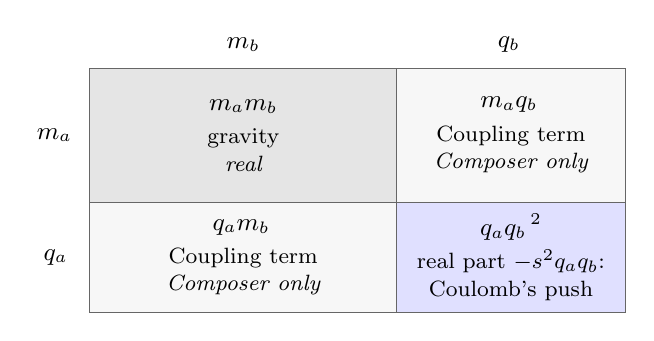
\begin{tikzpicture}[every node/.style={font=\small}]
  \def\wa{3.9}\def\wb{2.9}\def\ha{1.7}\def\hb{1.4}
  \fill[black!10] (0,0) rectangle (\wa,\ha);
  \fill[black!3] (\wa,0) rectangle ({\wa+\wb},\ha);
  \fill[black!3] (0,-\hb) rectangle (\wa,0);
  \fill[blue!12] (\wa,-\hb) rectangle ({\wa+\wb},0);
  \draw[black!60] (0,-\hb) rectangle ({\wa+\wb},\ha);
  \draw[black!60] (\wa,-\hb) -- (\wa,\ha);
  \draw[black!60] (0,0) -- ({\wa+\wb},0);
  \node at ({\wa/2},{\ha+0.3}) {$m_b$};
  \node at ({\wa+\wb/2},{\ha+0.3}) {$q_b\,\Gp$};
  \node[anchor=east] at (-0.1,{\ha/2}) {$m_a$};
  \node[anchor=east] at (-0.1,{-\hb/2}) {$q_a\,\Gp$};
  \node[align=center] at ({\wa/2},{\ha/2}) {$m_a m_b$\\[1pt] {\footnotesize gravity}\\[-1pt] {\footnotesize\itshape real}};
  \node[align=center] at ({\wa+\wb/2},{\ha/2}) {$m_a q_b\,\Gp$\\[1pt] {\footnotesize Coupling term}\\[-1pt] {\footnotesize\itshape Composer only}};
  \node[align=center] at ({\wa/2},{-\hb/2}) {$q_a m_b\,\Gp$\\[1pt] {\footnotesize Coupling term}\\[-1pt] {\footnotesize\itshape Composer only}};
  \node[align=center] at ({\wa+\wb/2},{-\hb/2}) {$q_a q_b\,\Gp^2$\\[1pt] {\footnotesize real part $-s^2 q_a q_b$:}\\[-1pt] {\footnotesize Coulomb's push}};
\end{tikzpicture}

\caption{The product of two cosmic masses, multiplied out as four rectangles (\cref{law:interaction,prop:law-real}). Mass times mass gives gravity. Each mass times the other body's charge gives the Coupling term, which lies along the Composer axis and has no real part. Charge times charge gives $q_a q_b\,\Gp^2$, whose real part is $-s^2 q_a q_b$ by the Rule of the Square: Coulomb's push, at every angle. The pieces are not drawn to scale.}
\label{fig:product}
\end{figure}

This is the real reading of \cref{def:real-reading} applied to one law (\cref{fig:product}). It reproduces Newton's and Coulomb's laws together, each with its own constant and its own sign, and adds nothing to them: a body at rest feels no new force.

\subsection{Why like charges push apart, at every angle}\label{subsec:why-sign}

In this framework the sign in \cref{def:reading} comes from the algebra of the plane. Had mass and charge been put into one real number, $\mu = m + \lambda q$ with a real $\lambda$ in kg\,C$^{-1}$, the product would be $\mu_a\mu_b = m_a m_b + \lambda(m_a q_b + q_a m_b) + \lambda^2 q_a q_b$. Since $\lambda^2 > 0$ for every $\lambda$, a law built on that product would pull two like charges together exactly as it pulls two masses. The choice $\lambda^2 = K/G$ gives the electric term Coulomb's strength, but no choice of $\lambda$ gives it Coulomb's sign. To carry both signs, the law needs a unit whose square points back along the mass axis.

\begin{proposition}[The sign of the interaction]\label{prop:sign}
In every true relative plane, whatever the angle $\pb$, the real part of the Cosmic Interaction Law is
\[
F = \frac{G\,m_a m_b - K\,q_a q_b}{r^2} .
\]
Two masses pull, two like charges push, and two unlike charges pull, each with the full strength of Newton's or Coulomb's law.
\end{proposition}

\begin{proof}
By the Rule of the Square~\cref{eq:square}, $\Re(\Gp^2) = -s^2$ for every $\pb$, so \cref{prop:law-real} holds with no condition on the angle; the signs follow from those of $m_a m_b \ge 0$ and of $q_a q_b$.
\end{proof}

The sign rests on one choice, the real reading (\cref{def:real-reading}); read by the shadow instead, it would depend on the angle (below).
 Given that reading, the minus sign is not put in by hand: it is the real coordinate of the square of the second unit, $-s^2$, which the Rule of the Square gives for every angle and every length~\citep[Proposition~4.1]{DerrazGN2026}. A reader may still say that writing a pair $(m, q)$ with the quadratic form $m_a m_b - s^2 q_a q_b$ builds the sign in, as a metric with one plus and one minus would. Our only reply is that here the form is the multiplication of a number system, a field, so that every rule of complex arithmetic applies to it (\cref{subsec:square,subsec:why-lean}); whether this is more than a choice of notation, the reader may judge.

\paragraph{Which root to draw.} The angle enters only through the other reading. By~\cref{eq:shadow}, the shadow of $\Gp$ is $\lvert\Gp\rvert\cos\pb$ and the shadow of $\Gp^2$ is $\lvert\Gp\rvert^2\cos 2\pb$, so that
\begin{equation}\label{eq:shadow-law}
G\,\Sh(\mu_a\mu_b) = G\,m_a m_b + \sqrt{KG}\,\cos\pb\,(m_a q_b + q_a m_b) + K\cos 2\pb\;q_a q_b .
\end{equation}
Read by its shadow, the electric term keeps only the share $\cos 2\pb$ of Coulomb's strength, and for like charges it has the sign of $\cos 2\pb$. At the arcsine root, $\cos 2\pb_1 \approx 0.93801$, and two like charges would pull. At the mirror root, $\cos 2\pb_2 \approx -0.93801$, the square of the Composer Unit leans at $159.72^\circ$ and points back along the mass axis, as it does for every angle between $\pi/4$ and $3\pi/4$~\citep[Theorem~3.7]{DerrazGN2026}, and like charges push in both readings. We therefore draw the frame at the mirror root, $\pb = 79.86^\circ$. The choice is a convention. The real reading, which is the one this paper uses (\cref{def:real-reading}), gives Coulomb's full strength and sign at every angle (\cref{prop:sign}), and at the drawn angle the shadow reading is excluded by experiment (\cref{subsec:coupling}). As far as this paper goes, the angle fixes only the Composer coordinate and the drawing of the frame.


